\documentclass[../main.tex]{subfiles}

\begin{document}
\subsection{Determinación de la masa del Cuerpo}
\begin{enumerate}
    \item Pasamos a traer los materiales a la mesa de trabajo.
    \item Se pesó las masas de los objetos en la balanza digital para saber la incertidumbre respectiva.
    \item Se colocó el objeto 1 (masa ploma) en el brazo mayor y una vez equilibrada la balanza se pasó a retirar el objeto 1.
    \item A continuación, se colocó los jinetillos en las ranuras del brazo mayor de tal manera que se llegue al equilibrio con el contrapeso.
    \item Se anotó las posiciones que ocupan los jinetillos a la tabla de datos. Y se siguieron los mismos pasos para el objeto 2 (masa dorada) y 3 (pelota de tecnopor).
\end{enumerate}

\subsection{Determinación del Empuje}
\begin{enumerate}
    \item Se llenó el recipiente grande con agua para luego ser ubicado en la balanza de brazos.
    \item Se colocó el objeto 1 en el brazo mayor y nos dimos cuenta que no se sumergía completamente en el agua, por lo cual se procedió a poner un soporte adecuado debajo del vaso grande.
    \item Una vez que sumergido completamente, se procedió a equilibrar usando el contrapeso.
    \item Luego se retiró la masa para ubicar los jinetillos en las ranuras de tal manera que se consiga el equilibrio nuevamente.
    \item Se anotó las posiciones que ocupan los jinetillos a la tabla de datos. Y se siguieron los mismos pasos para el objeto 2 (masa dorada).
    \item Para el objeto 3 (pelota de tecnopor) se enganchó el objeto 1 y 2 aumentando así su masa total. Y se siguió el mismo procedimiento anterior.
\end{enumerate}
  
\begin{figure}[H]
    \centering
    \begin{tabular}{c c}
        \centering
        \begin{subfigure}{0.4\linewidth}
            \centering
            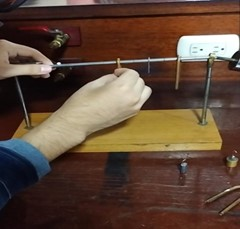
\includegraphics[width=0.4\linewidth]{resources/proc1.jpg}
            \caption{Colocación de los jinetillos.}
            \label{fig:proc1}
        \end{subfigure} &
        \begin{subfigure}{0.4\linewidth}
            \centering
            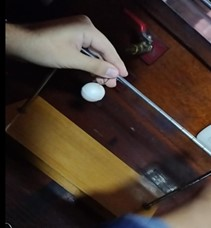
\includegraphics[width=0.4\linewidth]{resources/proc2.jpg}
            \caption{calibración de una masa.}
            \label{fig:proc2}
        \end{subfigure}\\
        \begin{subfigure}{0.4\linewidth}
            \centering
            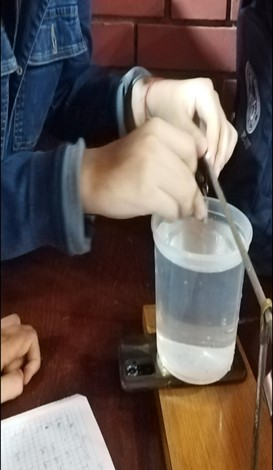
\includegraphics[width=0.4\linewidth,height=0.4\linewidth]{resources/proc3.jpg}
            \caption{Sumersión de una masa.}
            \label{fig:proc3}
        \end{subfigure}&
        \begin{subfigure}{0.4\linewidth}
            \centering
            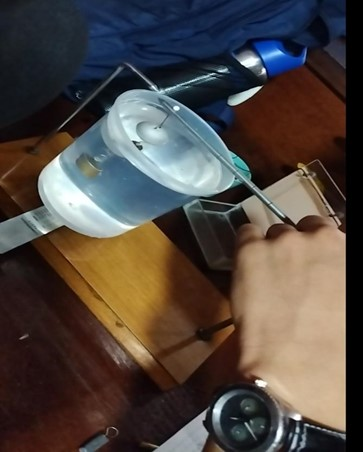
\includegraphics[width=0.4\linewidth]{resources/proc4.jpg}
            \caption{Calibración del contrapeso.}
            \label{fig:proc4}
        \end{subfigure}\\
    \end{tabular}
    \caption{Procedimiento Experimental de los experimentos 1 y 2}
    \label{fig:proc_exps}
\end{figure}
\end{document}
